\section{Results}
\label{sec:result}

The results compare network and corridor distributions built from the same
segments and examine how their relationship varies across services and
countries. Exposure measures how often a path enters the feasible inter-region
corridor space. Conditional breadth measures how candidate-bearing
observations are distributed within that space. We first establish these two
properties, then examine their geographic variation and the paired cross-layer
distributions.

The processing pipeline retains 490,911 valid traceroutes from 707,314 raw
records, yielding 3,291,063 atomic segments. Of the 2,432,559 mappable
segments, 555,119 reach candidate landing points, 171,232 satisfy the corridor
constraints, and 124,350 support inter-region corridors. The final set contains
71,990 single-corridor segments and 52,360 bounded multi-corridor segments.
Under the unit-mass aggregation rule, they form 370 auditable
country-measurement units.

\subsection{Service-Facing Paths Show Lower Candidate Exposure}
\label{subsec:overall-exposure}

DNS exposure has a pronounced upper tail: inter-region candidates appear
infrequently for most countries and recur in a smaller group. The DNS family
contains 945 country-measurement units with at least 30 valid traceroutes,
covering 77 countries. Pooling eligible Root observations within each country
by valid-trace count yields a median exposure of 5.50\% (IQR:
1.10\%-23.04\%; mean: 17.80\%). The difference between the median and mean
reveals this uneven distribution across countries.

The three application measurements occupy the same low-exposure range.
Median country-measurement exposure is 1.90\% for Wikipedia, 1.96\% for
Reddit, and 1.43\% for Netflix Assets. The multi-target topology references
reach 23.24\% for MSM~5051 and 23.81\% for MSM~5151. Figure
~\ref{fig:result-overview} compares the complete country distributions and
shows this separation.

Country-matched comparisons show lower DNS exposure while preserving source
geography and changing the target population. DNS exposure is lower than
MSM~5051 in 70 of 77 shared countries, with a median paired difference of
\(-14.52\) percentage points. It is lower than MSM~5151 in 54 of 59 shared
countries, with a median difference of \(-14.82\) points. The paired direction
holds for 90.9\% and 91.5\% of the shared countries, respectively.

The two protocols therefore reveal the same family ordering: service-facing
targets expose a smaller inter-region path population than the dynamic
multi-target measurements observed from the same countries.

\begin{figure*}[htb]
  \centering
  \subfloat[Country-measurement exposure.\label{fig:result-overview-distribution}]{%
    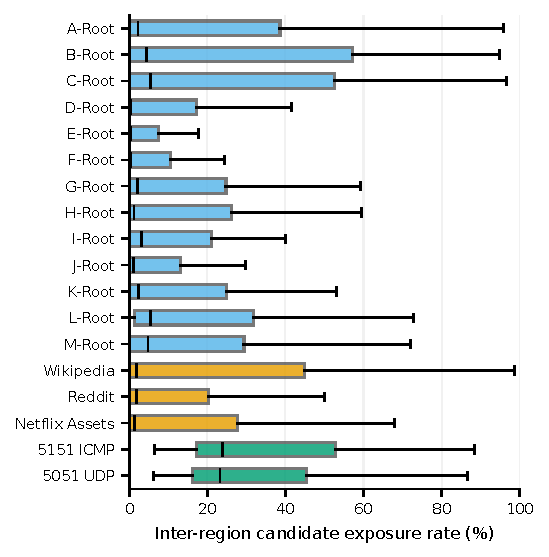
\includegraphics[width=0.39\textwidth]{figures/fig_result_overview_distribution.pdf}}
  \hspace{0.045\textwidth}
  \subfloat[Country-matched comparison.\label{fig:result-overview-paired}]{%
    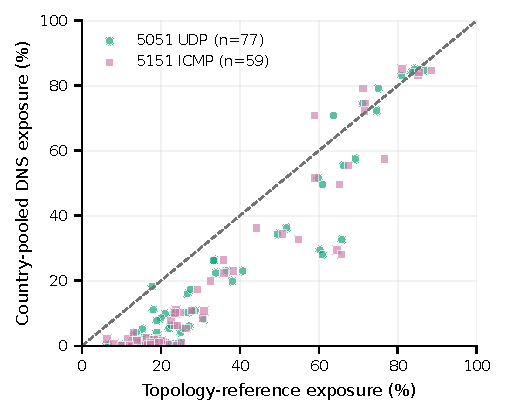
\includegraphics[width=0.34\textwidth]{figures/fig_result_overview_paired.pdf}}
  \caption{Inter-region candidate exposure.}
  \label{fig:result-overview}
\end{figure*}

\subsection{Service-Facing Observations Occupy Narrower Corridor Spaces}
\label{subsec:exposure-concentration}

We measure corridor breadth over 222 DNS Root, 53 application, and 95
topology-reference units. Every unit meets the audit thresholds in
Section~\ref{sec:framework_path_segmentation}. Its network and corridor
distributions contain the same candidate-bearing segments. Table
~\ref{tab:family-summary} reports the median concentration and breadth of
each family.

\begin{table*}[htb]
  \centering
  \caption{Network-transition and corridor distributions.}
  \label{tab:family-summary}
  \footnotesize
  \setlength{\tabcolsep}{4.0pt}
  \begin{tabular}{lrrrrrr}
    \toprule
    Family & Units & Net. Top-2 & Corr. Top-2 & \(\Delta\)Top-2
      & Eff. network & Eff. corridor \\
    \midrule
    DNS Roots & 222 & 53.1\% & 72.0\% & +11.0 pp & 7.45 & 3.84 \\
    Applications & 53 & 45.2\% & 70.3\% & +21.0 pp & 9.89 & 3.51 \\
    Topology references & 95 & 27.3\% & 30.6\% & +2.7 pp & 24.34 & 18.01 \\
    \bottomrule
  \end{tabular}
\end{table*}

DNS Roots and applications occupy narrower corridor spaces than the topology
references. Their median corridor Top-2 shares are 72.0\% and 70.3\%,
compared with 30.6\% for topology references; their effective corridor counts
are 3.84 and 3.51, compared with 18.01. The topology-reference median thus
contains 4.7 times as many effective corridors as DNS and 5.1 times as many as
the applications. Its Top-2 share is 41.4 percentage points below DNS and
39.7 points below the applications.

The high-concentration tail follows the same family ordering. The leading two
corridors receive at least 80\% of mass in 83 of 222 DNS units (37.4\%),
16 of 53 application units (30.2\%), and 4 of 95 topology-reference units
(4.2\%). These threshold counts and the family medians describe the
separation at the upper end and center of the concentration distributions,
respectively.

The three applications reach similar absolute corridor breadth through
different amounts of redistribution from their network-transition
distributions. Wikipedia, Reddit, and Netflix Assets have median corridor
Top-2 shares of 68.3\%, 71.0\%, and 71.6\%, with 4.25, 3.25, and 3.47
effective corridors. Their median Top-2 shifts are 11.0, 25.6, and 23.6
percentage points, respectively. Together, these measurements describe their
shared narrow physical footprint and different cross-layer shifts.

Figure~\ref{fig:corridor-breadth} shows that the family separation extends
across the distributions. The service-facing ECDFs occupy the
higher-concentration range, and their effective-count distributions remain
centered on three to four equally weighted corridors. Top-2 share captures
mass in the dominant directions, while effective count captures breadth across
the full support. Both metrics yield the same family ordering.

\begin{figure*}[htb]
  \centering
  \subfloat[Corridor Top-2 share.\label{fig:corridor-top2-ecdf}]{%
    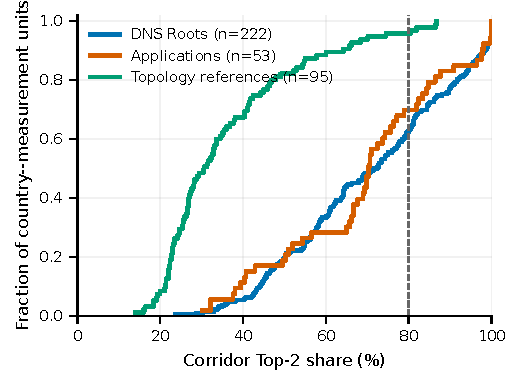
\includegraphics[width=0.36\textwidth]{figures/fig_corridor_concentration_ecdf.pdf}}
  \hspace{0.05\textwidth}
  \subfloat[Effective category counts.\label{fig:effective-counts}]{%
    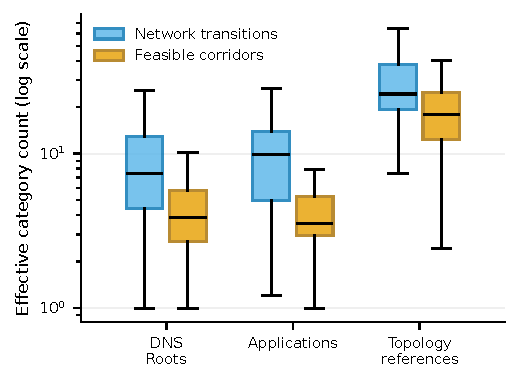
\includegraphics[width=0.36\textwidth]{figures/fig_effective_count_comparison.pdf}}
  \caption{Corridor concentration and breadth by measurement family.}
  \label{fig:corridor-breadth}
\end{figure*}

The largest family difference remains the absolute physical breadth reached
after projection. Normalized entropy provides a support-relative view:
median entropy reduction is 0.126 for DNS Roots, 0.164 for applications, and
0.081 for topology references. Service-facing paths repeatedly occupy a
smaller feasible-corridor space, while the multi-target references distribute
observations over many more coastal directions.

\subsection{Geography Separates Exposure from Concentration}
\label{subsec:geography}

We compare geography at the country level, giving equal weight to countries
represented by different numbers of Root measurements. Following Liu et
al.~\cite{liu2020outofsight}, probe countries are grouped as island or
archipelagic, landlocked, and other coastal. Each country contributes one
pooled DNS exposure observation and the median corridor distribution over its
auditable DNS units.

Island and archipelagic countries form the highest-exposure group. Their
median country-pooled DNS exposure is 49.61\% across 9 countries, compared
with 7.88\% for 54 other coastal countries and 1.70\% for 14 landlocked
countries. This ordering describes how frequently observed Root paths enter
an inter-region candidate space.

Conditional corridor breadth follows a different ordering. Island and
archipelagic countries have a median Top-2 corridor share of 53.3\% and
5.58 effective corridors. Other coastal countries reach 75.4\% and 3.39.
The two represented landlocked countries reach 80.2\% and 2.51. Figure
~\ref{fig:country-geography} presents both distributions together with the
contributing country counts.

Across the 38 countries with both pooled exposure and an auditable corridor
summary, more frequent entry into the candidate space tends to accompany
broader conditional support. Exposure and corridor Top-2 share have a
Spearman rank association of \(-0.29\); exposure and effective corridor count
have the corresponding association of 0.30. The country-level ordering thus
follows the geographic group result.

\begin{figure*}[htb]
  \centering
  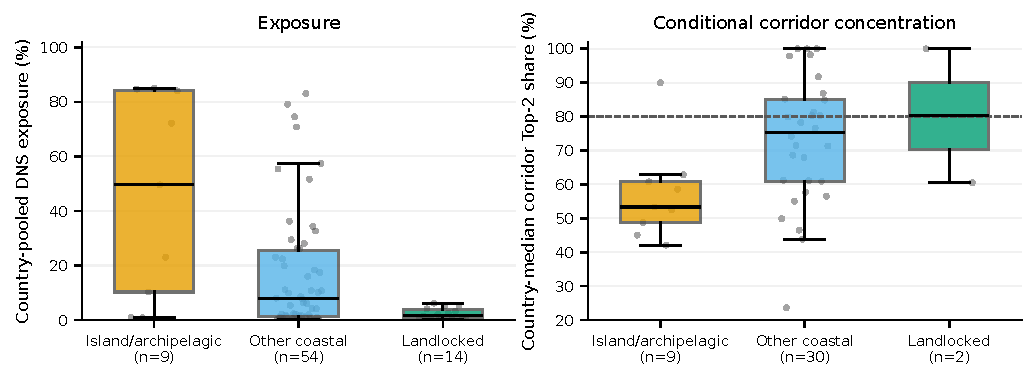
\includegraphics[width=0.72\textwidth]{figures/fig_country_geography_30km.pdf}
  \caption{DNS exposure and corridor concentration by geography.}
  \label{fig:country-geography}
\end{figure*}

Geography therefore separates exposure from conditional corridor breadth.
Island and archipelagic countries enter the candidate space more frequently,
yet their candidate-bearing observations span more coastal directions. Other
coastal countries enter less frequently and concentrate more strongly once
exposure occurs. Exposure records the frequency of submarine involvement;
corridor breadth describes the physical directions supporting that
involvement.

\subsection{Cross-Layer Contraction Is Heterogeneous}
\label{subsec:cross-layer}

DNS and application units shift upward more strongly than topology references
in the paired network-transition and corridor Top-2 comparison. Figure
~\ref{fig:cross-layer} shows all 370 auditable units. The common 80\% lines
organize the distributions into four descriptive classes, and the diagonal
separates increases in corridor concentration from decreases.

\begin{figure*}[htb]
  \centering
  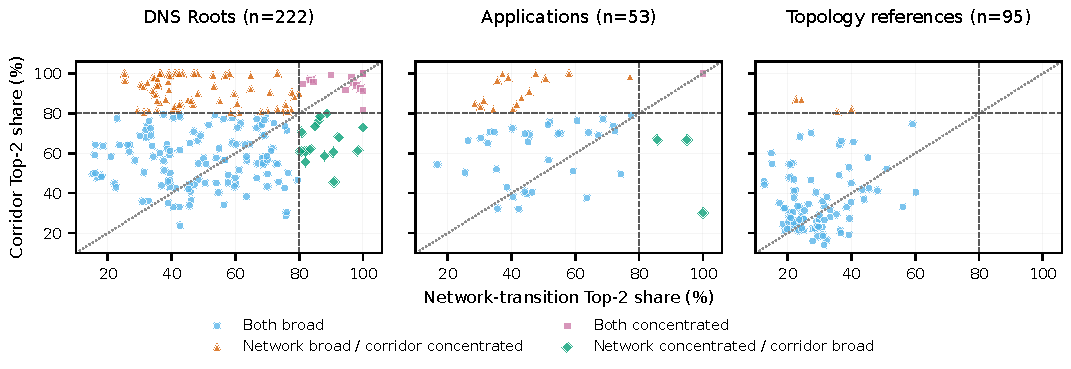
\includegraphics[width=0.92\textwidth]{figures/fig_cross_layer_distribution.pdf}
  \caption{Network-transition and corridor Top-2 shares.}
  \label{fig:cross-layer}
\end{figure*}

Contraction is a recurring service-facing pattern, while broad support at
both layers remains the largest service-facing class. Among 275
service-facing units, 81 (29.5\%) are network-broad/corridor-concentrated,
158 (57.5\%) remain broad at both layers, 18 (6.5\%) are concentrated at
both, and 18 (6.5\%) are network-concentrated/corridor-broad. Four of 95
topology-reference units (4.2\%) enter the contraction class; the other 91
remain broad at both layers.

DNS and applications enter the contraction class at similar rates but show
different median continuous shifts. The class contains 66 of 222 DNS units
(29.7\%) and 15 of 53 application units (28.3\%). Their median continuous
Top-2 shifts are 11.0 and 21.0 percentage points, respectively. Application
units cross the 80\% boundary at a similar frequency and redistribute more
mass toward their two leading corridors. Continuous shifts also reveal
substantial narrowing within the broad-broad class.

Continuous metrics identify redistribution toward fewer leading physical
directions both within and across the threshold classes. Across the
service-facing population, corridor Top-2 share increases in 184 of 275
units (66.9\%), and effective category count contracts in 204 (74.2\%). Of
the 239 units with a broad network distribution, 178 (74.5\%) move upward
in Top-2 share: 81 cross the concentration threshold, while 97 remain broad
at both layers with a median increase of 6.3 percentage points.

Three cases distinguish continuous narrowing, expansion, and changes in
absolute breadth from support-relative evenness.
\textbf{Singapore-Netflix} moves from 32.5\% network Top-2 share to 65.0\%
corridor Top-2 share, while its effective count contracts from 19.86 to
3.41. It exhibits strong continuous narrowing while remaining below the
80\% boundary.

\textbf{New Zealand-Netflix} shows corridor expansion. Its share moves
from 63.6\% to 37.6\%, with effective count expanding from 5.18 to 6.92.

\textbf{Singapore-H-Root} separates absolute breadth from support-relative
evenness. Its share moves from 39.6\% to 50.1\%, and its effective
count contracts from 20.67 to 5.99, while normalized entropy changes only
slightly.

Repeated overlap among bounded multi-corridor sets produces the aggregate
distributions in these cases. Bounded multi-corridor segments account for
99.9\% of candidate-bearing observations in Singapore-Netflix, 78.1\% in
New Zealand-Netflix, and 98.2\% in Singapore-H-Root. Under the same
projection and aggregation rules, the cases show contraction, expansion,
and metric-specific change.

Service-facing measurements enter the inter-region candidate space less often
and occupy narrower corridor distributions than the topology references.
Within the service-facing population, country-service units span contraction,
preservation, and expansion. Network diversity and physical-corridor diversity
therefore describe distinct properties of application reachability.